

\begin{center}
\thispagestyle{empty}
%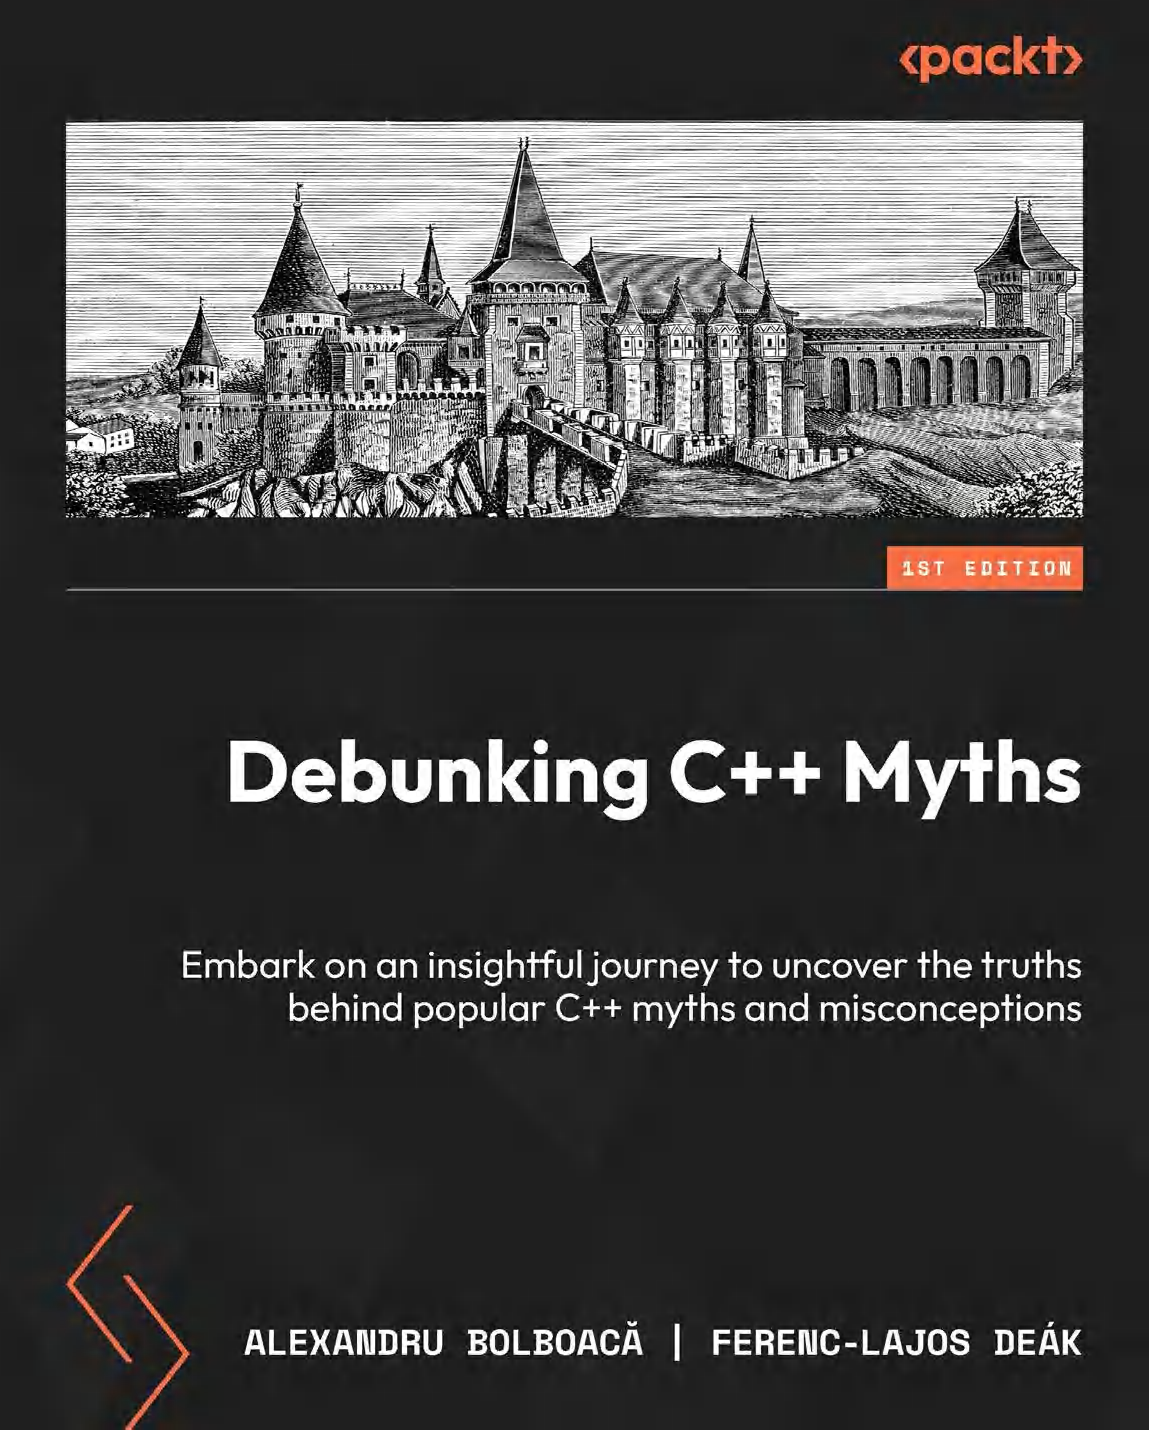
\includegraphics[width=\textwidth,height=\textheight,keepaspectratio]{cover.png}
\begin{tikzpicture}[remember picture, overlay, inner sep=0pt]
\node at (current page.center)
{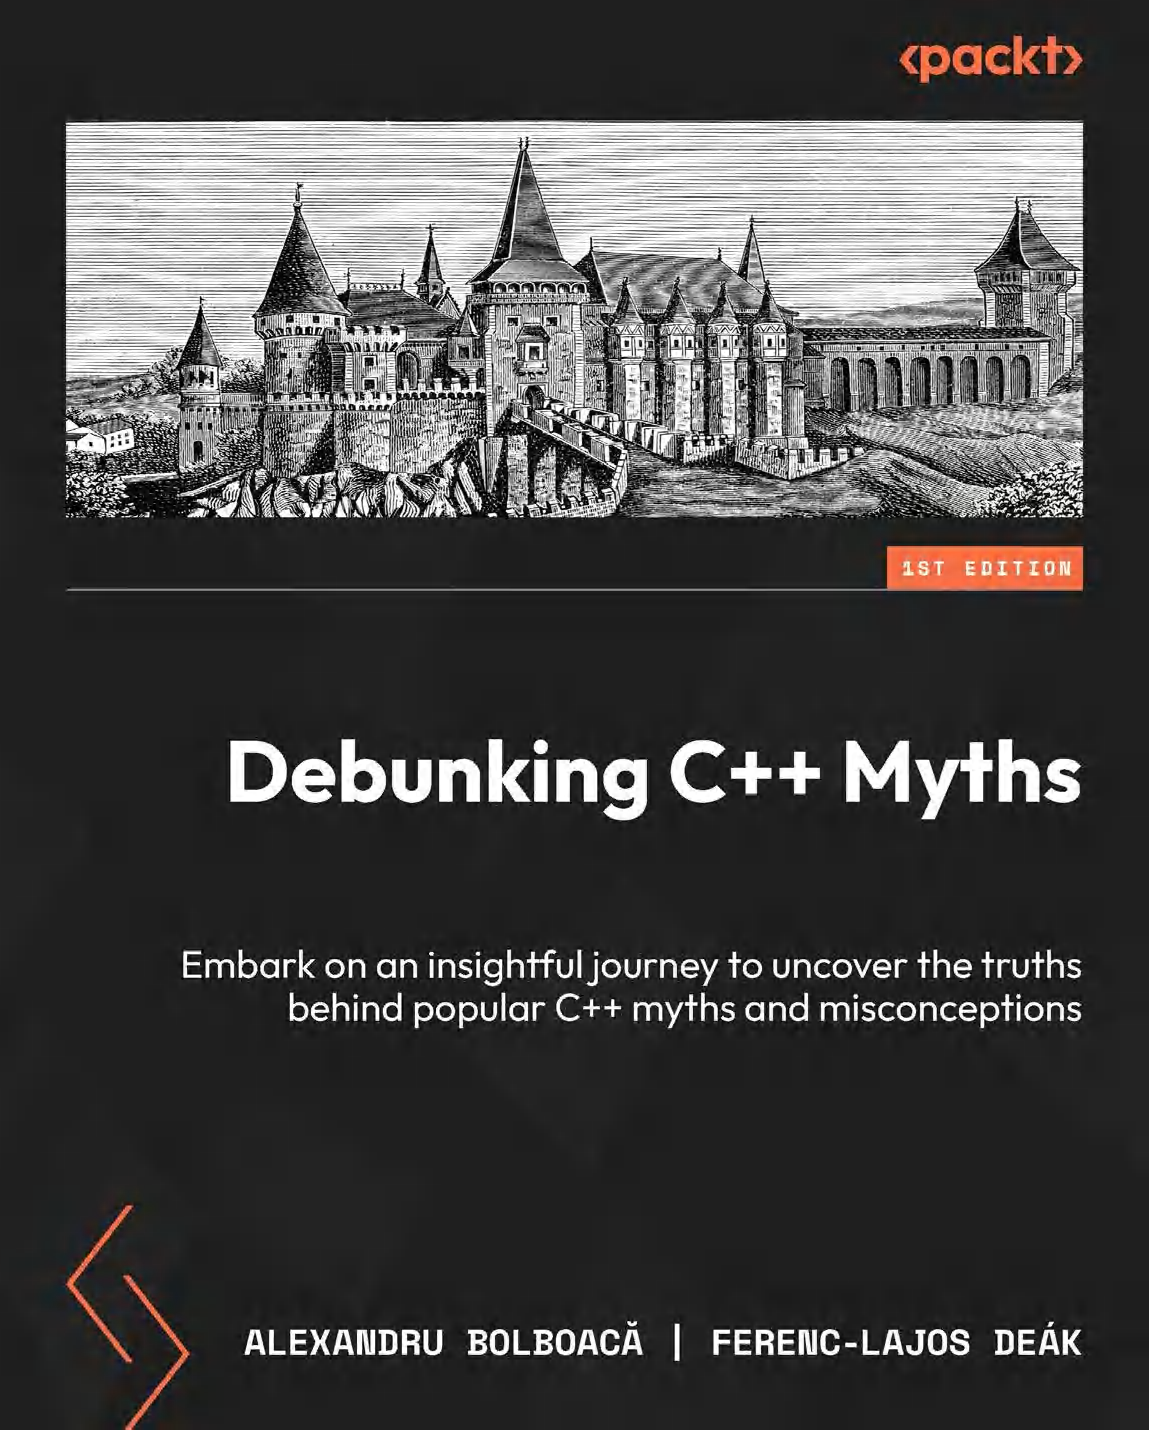
\includegraphics[width=\paperwidth, keepaspectratio=false]{cover.png}};
\end{tikzpicture}
\newpage
\thispagestyle{empty}
\huge
\textbf{消除C++迷思}
\\[9pt]
\normalsize
开启一段富有洞见的旅程,揭开 C++ 迷思与误解背后的真相
\\[9pt]
\normalsize
作者: Alexandru Bolboacă, Ferenc-Lajos Deák
\\[8pt]
\normalsize
译者:\href{https://github.com/xiaoweiChen/Debunking-Cpp-Myths}{陈晓伟}
\\[8pt]
\end{center}

\newpage

\begin{comment}
\end{comment}

\pagestyle{empty}
\tableofcontents
\newpage

\setsecnumdepth{section}

\myChapter{致谢}{}{content/dedicated.tex}
\newpage

\myChapter{关于作者}{}{content/about-the-author.tex}
\newpage

\myChapter{关于评审}{}{content/about-the-reviewer.tex}
\newpage

\myChapter{前言}{}{content/preface.tex}
\newpage

\myChapter{第1章}{C++很难学}{content/chapter1/0.tex}
\mySubsection{1.1.}{环境要求}{content/chapter1/1.tex}
\mySubsection{1.2.}{为什么 C++ 被认为很难学习?}{content/chapter1/2.tex}
\mySubsection{1.3.}{C++ 的难点以及如何掌握它们}{content/chapter1/3.tex}
\mySubsection{1.4.}{The Stroustrup method for learning C++}{content/chapter1/4.tex}
\mySubsection{1.5.}{The Kate Gregory method – don’t teach C}{content/chapter1/5.tex}
\mySubsection{1.6.}{The test-driven method for learning C++}{content/chapter1/6.tex}
\mySubsection{1.7.}{With great power…}{content/chapter1/7.tex}
\mySubsection{1.8.}{总结}{content/chapter1/8.tex}
\newpage

\myChapter{第2章}{Every C++ Program Is tandard-Compliant}{content/chapter2/0.tex}
\mySubsection{2.1.}{环境要求}{content/chapter2/1.tex}
\mySubsection{2.2.}{Somewhere in Ghana, far, far away}{content/chapter2/2.tex}
\mySubsection{2.3.}{Microsoft’s tiny, squishy C++}{content/chapter2/3.tex}
\mySubsection{2.4.}{The realm of free compilers}{content/chapter2/4.tex}
\mySubsection{2.5.}{When the header is not even C++}{content/chapter2/5.tex}
\mySubsection{2.6.}{The curious case of C++ locked in a box}{content/chapter2/6.tex}
\mySubsection{2.7.}{Past days of future C++}{content/chapter2/7.tex}
\mySubsection{2.8.}{总结}{content/chapter2/8.tex}
\newpage

\myChapter{第3章}{There’s a Single C++, nd It Is Object-Oriented}{content/chapter3/0.tex}
\mySubsection{3.1.}{环境要求}{content/chapter3/1.tex}
\mySubsection{3.2.}{The multiple facets of C++}{content/chapter3/2.tex}
\mySubsection{3.3.}{Functional programming in C++}{content/chapter3/3.tex}
\mySubsection{3.4.}{Metaprogramming}{content/chapter3/4.tex}
\mySubsection{3.5.}{Strong types to the limit}{content/chapter3/5.tex}
\mySubsection{3.6.}{What about ignoring types?}{content/chapter3/6.tex}
\mySubsection{3.7.}{总结}{content/chapter3/7.tex}
\newpage

\myChapter{第4章}{The Main() Function is the ntry Point to Your Application}{content/chapter4/0.tex}
\mySubsection{4.1.}{The main() function}{content/chapter4/1.tex}
\mySubsection{4.2.}{The penguin farm}{content/chapter4/2.tex}
\mySubsection{4.3.}{Let’s open the Windows (unless you’re on ISS)}{content/chapter4/3.tex}
\mySubsection{4.4.}{总结}{content/chapter4/4.tex}
\newpage

\myChapter{第5章}{In a C++ Class, rder Must There Be}{content/chapter5/0.tex}
\mySubsection{5.1.}{Size does matter}{content/chapter5/1.tex}
\mySubsection{5.2.}{The order that must be respected}{content/chapter5/2.tex}
\mySubsection{5.3.}{Deep thoughts about order}{content/chapter5/3.tex}
\mySubsection{5.4.}{The dark orders of C++}{content/chapter5/4.tex}
\mySubsection{5.5.}{When order does not matter}{content/chapter5/5.tex}
\mySubsection{5.6.}{总结}{content/chapter5/6.tex}
\newpage

\myChapter{第6章}{C++ Is Not Memory-Safe}{content/chapter6/0.tex}
\mySubsection{6.1.}{环境要求}{content/chapter6/1.tex}
\mySubsection{6.2.}{Memory safety is important}{content/chapter6/2.tex}
\mySubsection{6.3.}{The memory safety problems of older C++}{content/chapter6/3.tex}
\mySubsection{6.4.}{Modern C++ to the rescue}{content/chapter6/4.tex}
\mySubsection{6.5.}{The limits of modern C++}{content/chapter6/5.tex}
\mySubsection{6.6.}{There’s still more to do}{content/chapter6/6.tex}
\mySubsection{6.7.}{总结}{content/chapter6/7.tex}
\newpage

\myChapter{第7章}{There’s No Simple ay to Do Parallelism and oncurrency in C++}{content/chapter7/0.tex}
\mySubsection{7.1.}{环境要求}{content/chapter7/1.tex}
\mySubsection{7.2.}{Defining parallelism and concurrency}{content/chapter7/2.tex}
\mySubsection{7.3.}{Common issues with parallelism and concurrency}{content/chapter7/3.tex}
\mySubsection{7.4.}{Functional programming to the rescue!}{content/chapter7/4.tex}
\mySubsection{7.5.}{The Actor Model}{content/chapter7/5.tex}
\mySubsection{7.6.}{What we can’t do yet}{content/chapter7/6.tex}
\mySubsection{7.7.}{总结}{content/chapter7/7.tex}
\newpage

\myChapter{第8章}{The Fastest C++ ode is Inline Assembly}{content/chapter8/0.tex}
\mySubsection{7.1.}{Light me a pixel}{content/chapter8/1.tex}
\mySubsection{7.2.}{The sum of all numbers}{content/chapter8/2.tex}
\mySubsection{7.3.}{One instruction to rule them all}{content/chapter8/3.tex}
\mySubsection{7.4.}{总结}{content/chapter8/4.tex}
\newpage

\myChapter{第9章}{C++ Is Beautiful}{content/chapter9/0.tex}
\mySubsection{7.1.}{In search of beauty}{content/chapter9/1.tex}
\mySubsection{7.2.}{The definition of zero}{content/chapter9/2.tex}
\mySubsection{7.3.}{A parenthesis concerning parentheses}{content/chapter9/3.tex}
\mySubsection{7.4.}{C++uties}{content/chapter9/4.tex}
\mySubsection{7.5.}{总结}{content/chapter9/5.tex}
\newpage

\myChapter{第10章}{There Are No Libraries For odern Programming in C++}{content/chapter10/0.tex}
\mySubsection{7.1.}{How can we tell?}{content/chapter10/1.tex}
\mySubsection{7.2.}{A modern developer’s experience}{content/chapter10/2.tex}
\mySubsection{7.3.}{Common needs}{content/chapter10/3.tex}
\mySubsection{7.4.}{Compatibility}{content/chapter10/4.tex}
\mySubsection{7.5.}{Supply chain security}{content/chapter10/5.tex}
\mySubsection{7.6.}{总结}{content/chapter10/6.tex}
\newpage

\myChapter{第11章}{C++ Is Backward ompatible ...Even with C}{content/chapter11/0.tex}
\mySubsection{7.1.}{Is C really forward-compatible with C++?}{content/chapter11/1.tex}
\mySubsection{7.2.}{Whitespace matters – until it doesn’t}{content/chapter11/2.tex}
\mySubsection{7.3.}{The auto surprise}{content/chapter11/3.tex}
\mySubsection{7.4.}{总结}{content/chapter11/4.tex}
\newpage

\myChapter{第12章}{Rust Will Replace C++}{content/chapter12/0.tex}
\mySubsection{7.1.}{环境要求}{content/chapter12/1.tex}
\mySubsection{7.2.}{Why the competition?}{content/chapter12/2.tex}
\mySubsection{7.3.}{Core features of Rust}{content/chapter12/3.tex}
\mySubsection{7.4.}{Rust’s advantages}{content/chapter12/4.tex}
\mySubsection{7.5.}{Where C++ is better}{content/chapter12/5.tex}
\mySubsection{7.6.}{What C++ still needs}{content/chapter12/6.tex}
\mySubsection{7.7.}{总结}{content/chapter12/7.tex}
\newpage

\begin{comment}
\end{comment}
